\chapter{メタデータ編集}
IUGONETプロジェクトでは、IUGONET共通メタデータフォーマットに則ったメタデータを円滑に作成するためのツール
、すなわち{\bf IUGONETメタデータ・エディター}を提供しています。これは、フリーソフトであるEclipseをベースとし、
IUGONETメタデータ共通メタデータの為のXML Schema、XML形式のサンプル
・メタデータをパッケージ化したツールです。このツールを使うことにより、
通常のテキストエディターを用いた編集より、手早く確実にメタデータを
作成することが出来ます。

\section{IUGONETメタデータ・エディターのダウンロード}
初めに、
\begin{screen}
\begin{verbatim}
http://www.iugonet.org/iugonetmetadataeditor.html
\end{verbatim}
\end{screen}
から、PC環境に合わせて、
\begin{screen}
\begin{itemize}
\item iugonet-metadata-eidtor-win32.zip
\item iugonet-metadata-editor-macosx32.zip
\item iugonet-metadata-editor-linux32.zip
\end{itemize}
\end{screen}
のいずれかをダウンロードし、zipファイルを展開してください。

\section{IUGONETメタデータ・エディターの起動}
展開したzipファイルの中から、
\begin{screen}
\begin{verbatim}
iugonet
\end{verbatim}
\end{screen}
を実行すると、図\ref{IugonetMetadataEditor1}の通りに
IUGONETメタデータ・エディターが起動します。

\begin{figure}[H]
\begin{center}
\fbox{
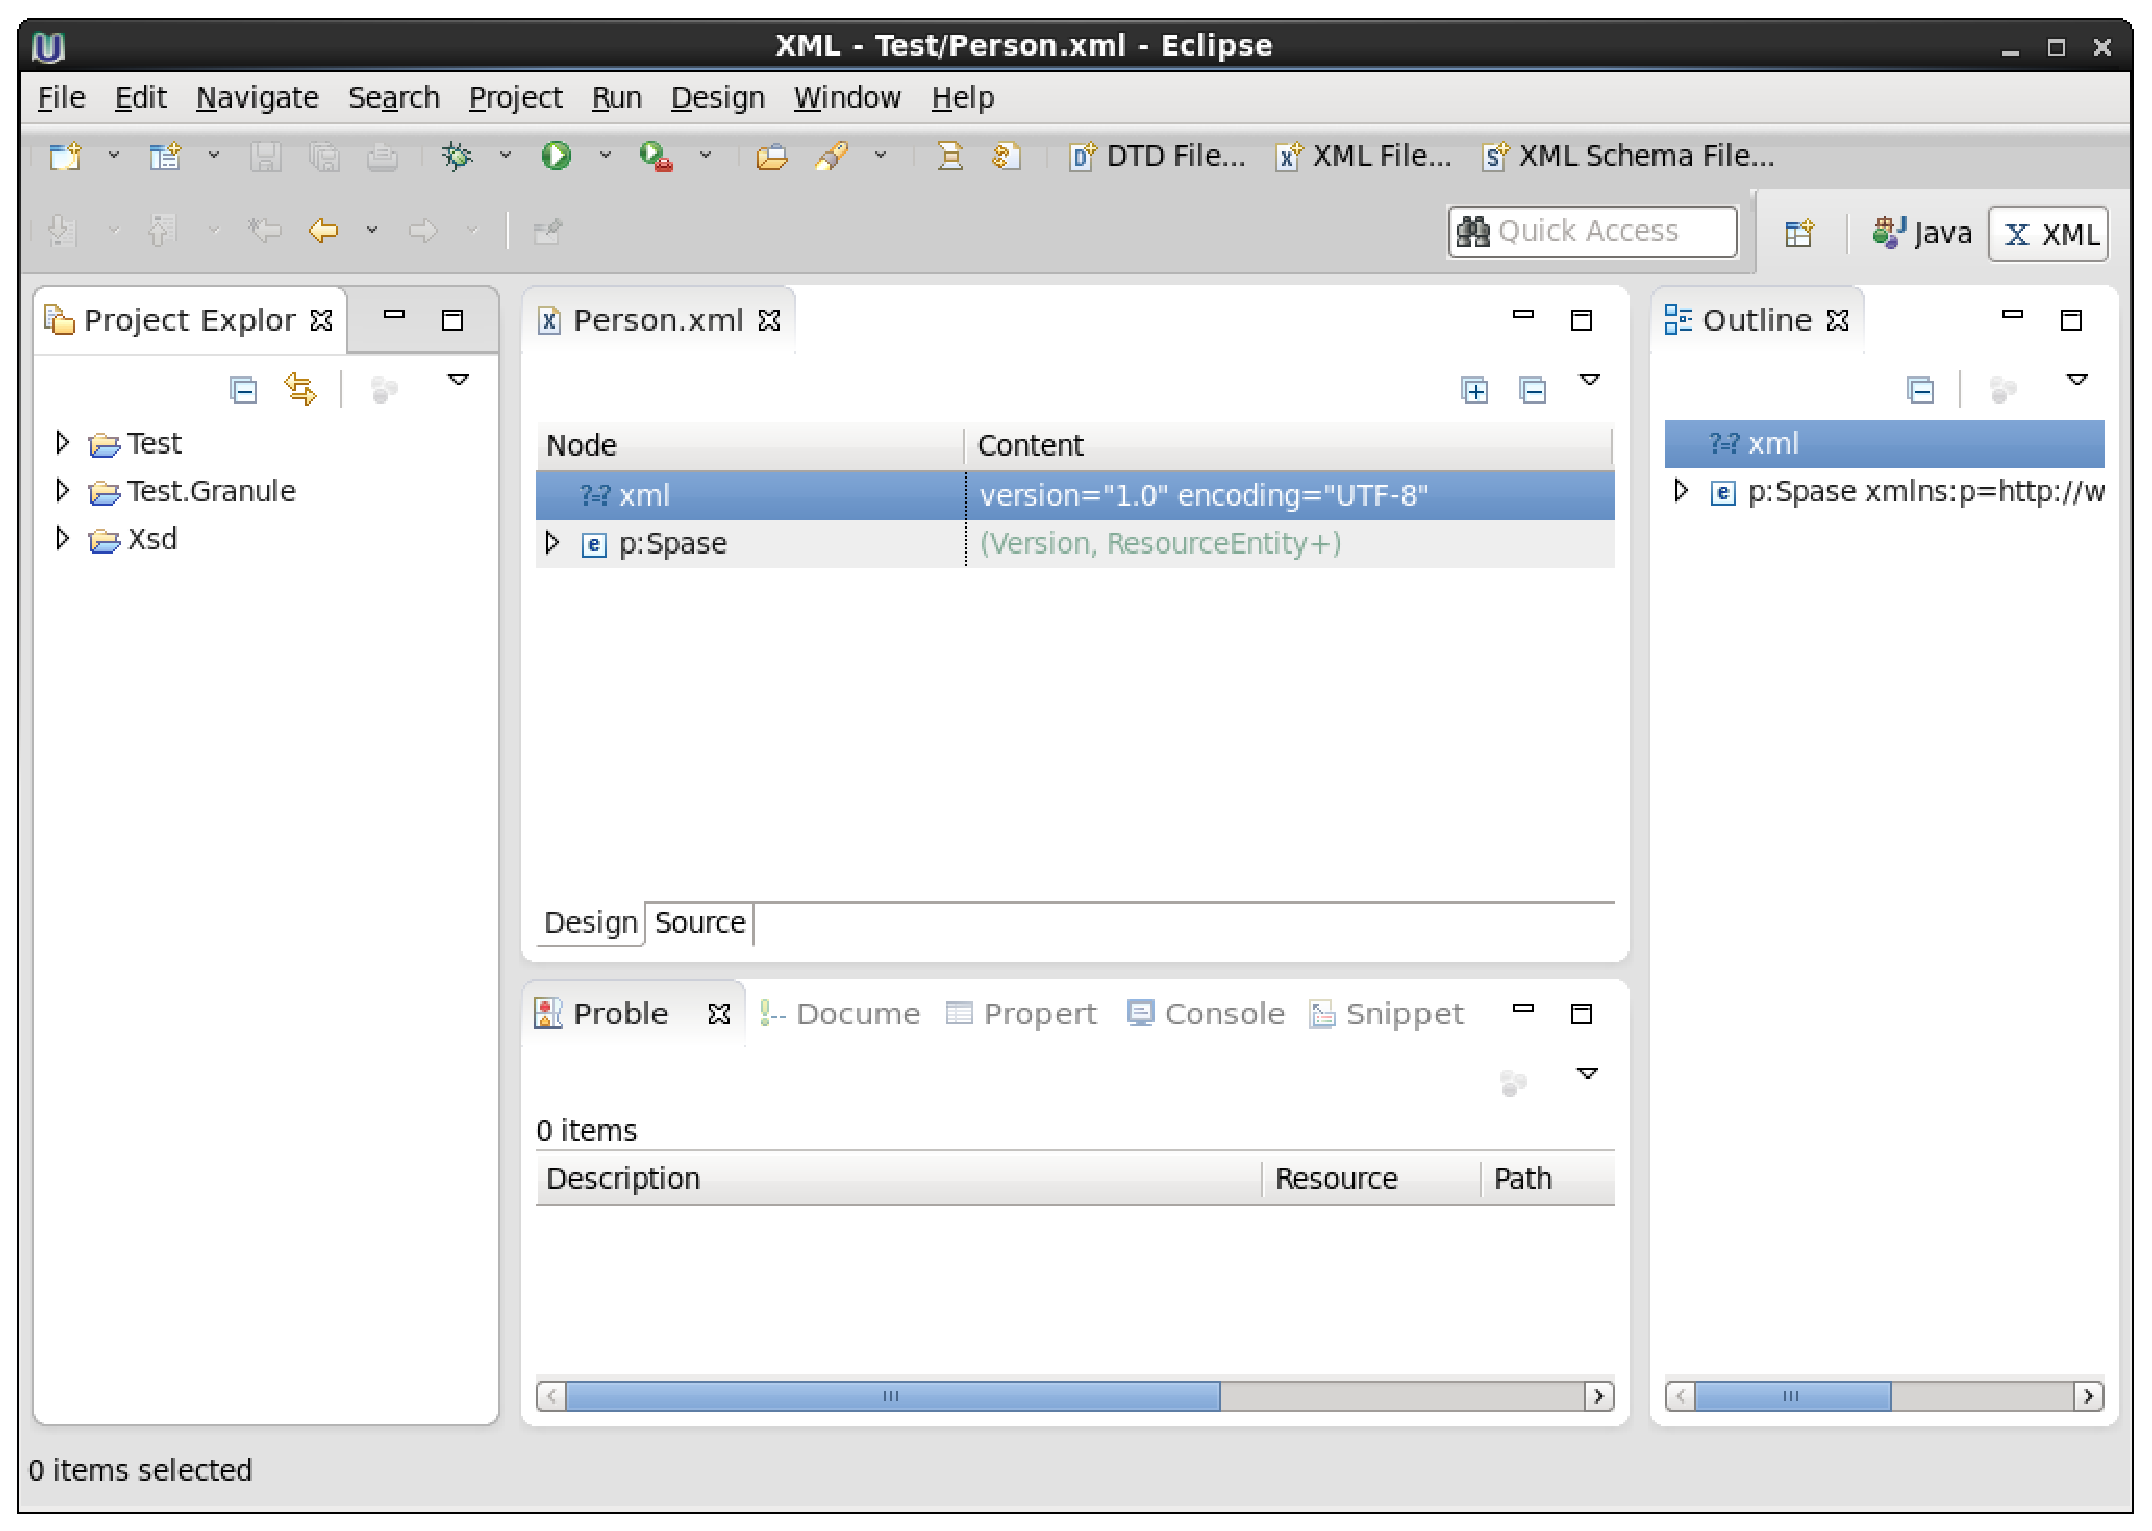
\includegraphics[width=12cm]{images/IugonetMetadataEditor1.eps}
}
\caption{IUGONETメタデータ・エディター起動画面。}
\label{IugonetMetadataEditor1}
\end{center}
\end{figure}

\subsection{メタデータ・ファイルの編集}

\subsubsection{Personの編集}

\begin{figure}[H]
\begin{center}
\fbox{
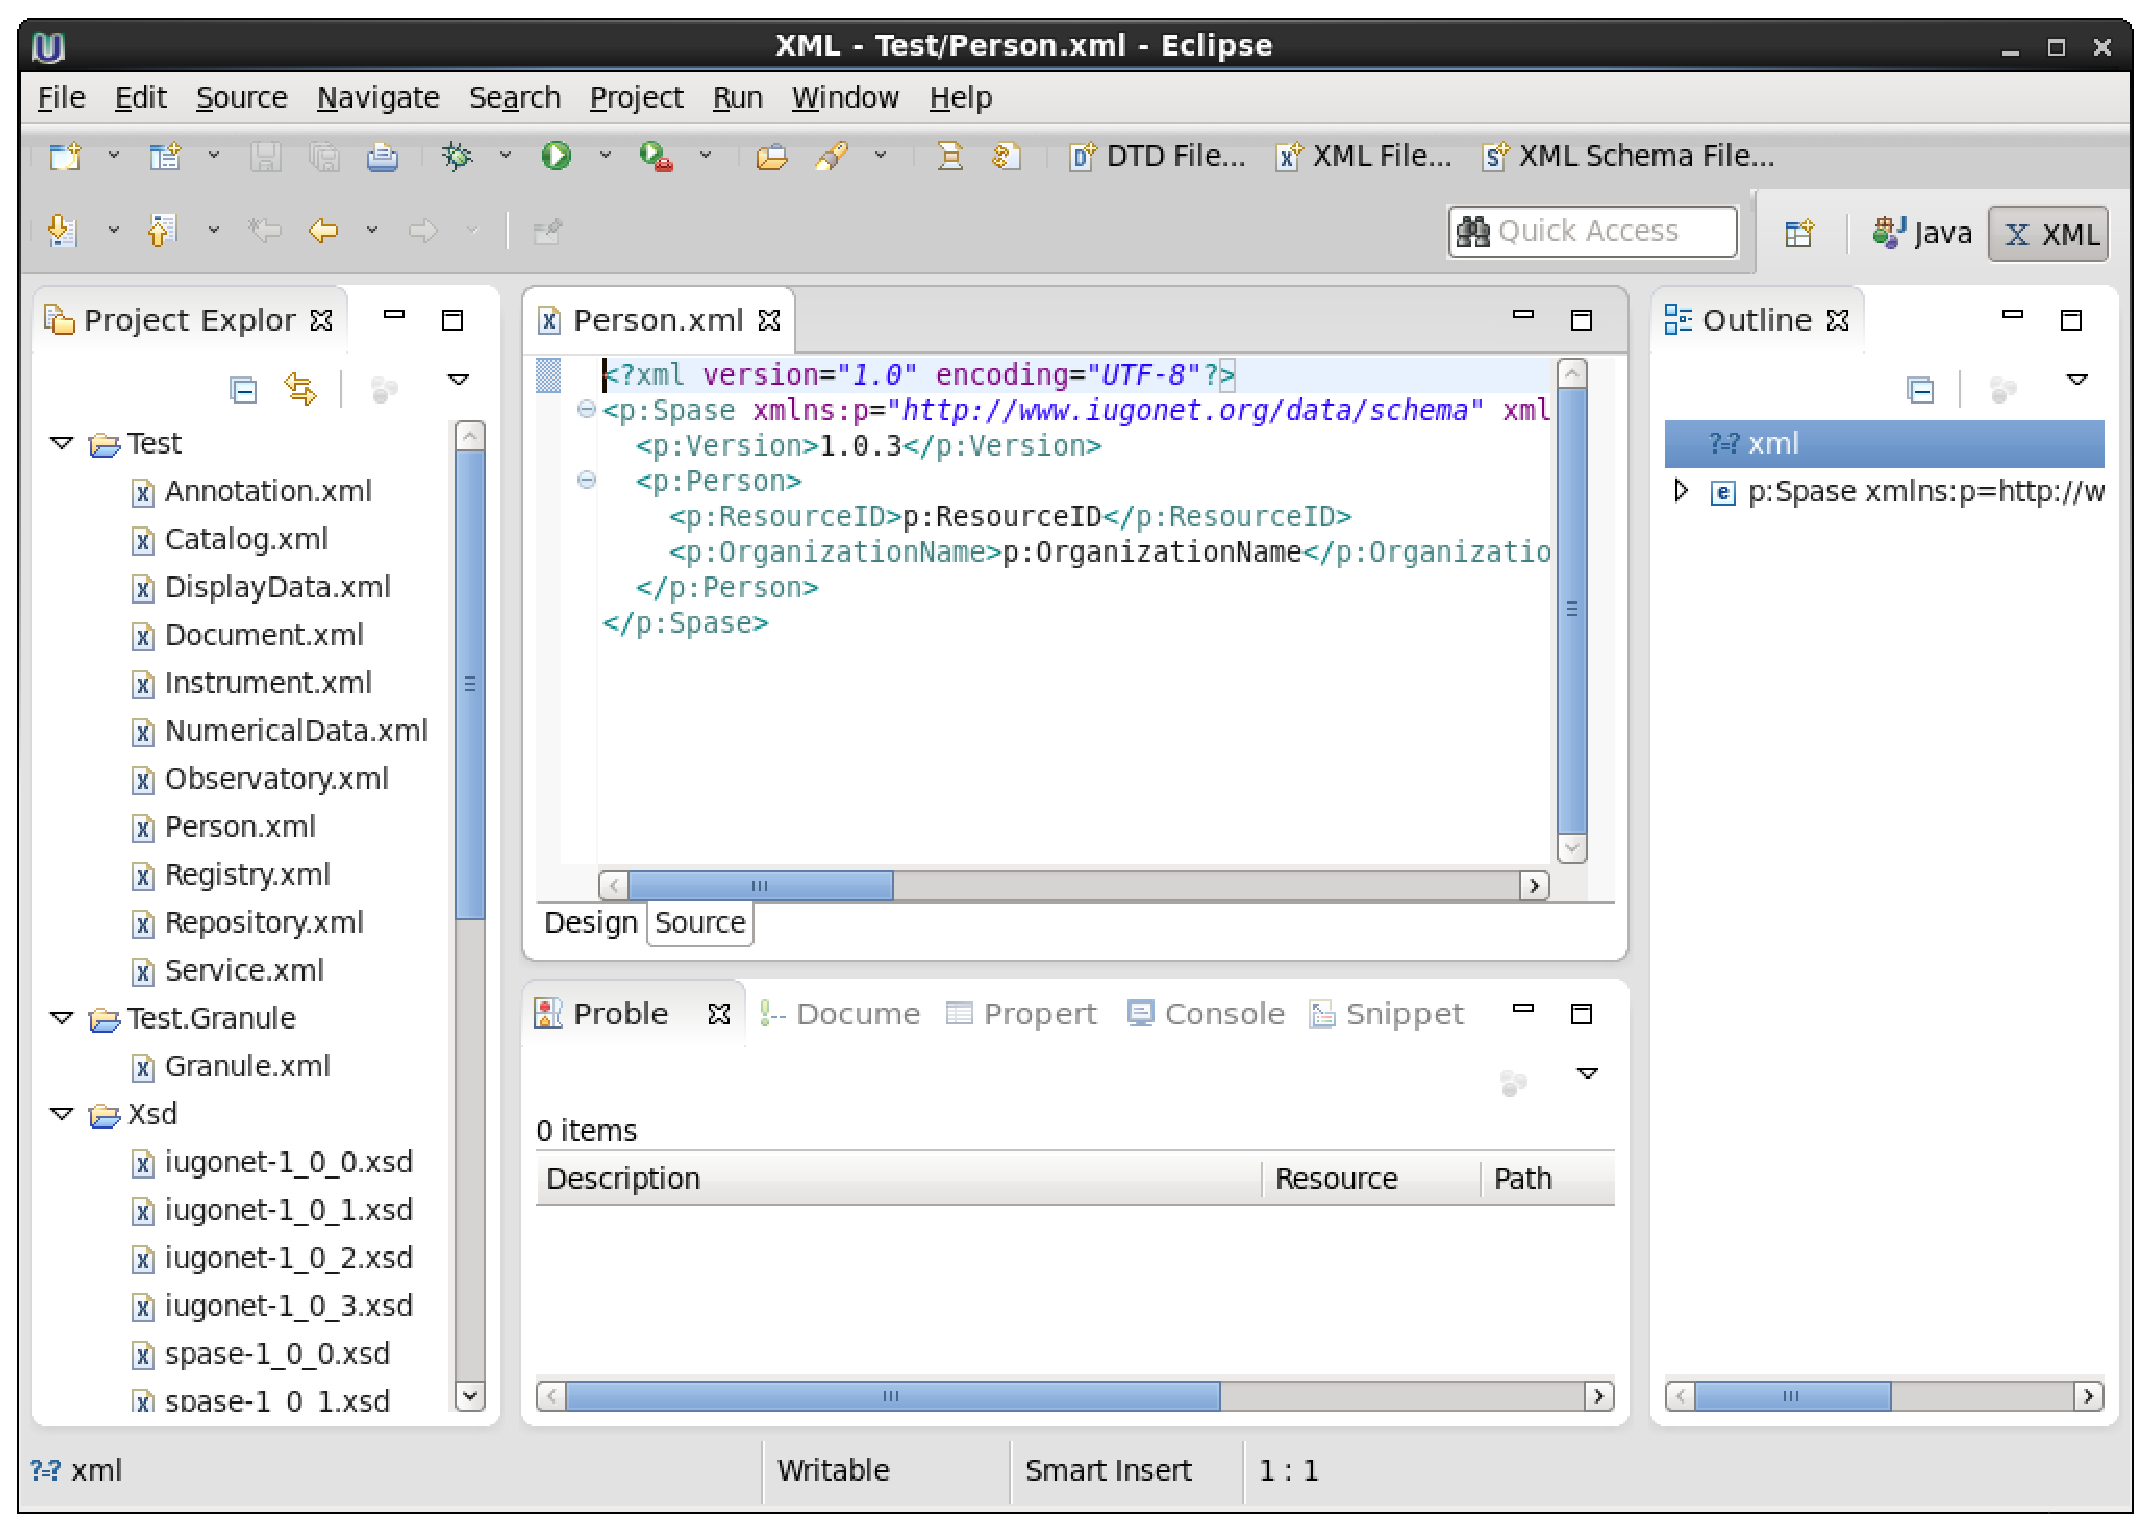
\includegraphics[width=12cm]{images/IugonetMetadataEditor2.eps}
}
\caption{Person.xml編集画面(Designタブ選択時)。}
\label{IugonetMetadataEditor2}
\end{center}
\end{figure}

\begin{figure}[H]
\begin{center}
\fbox{
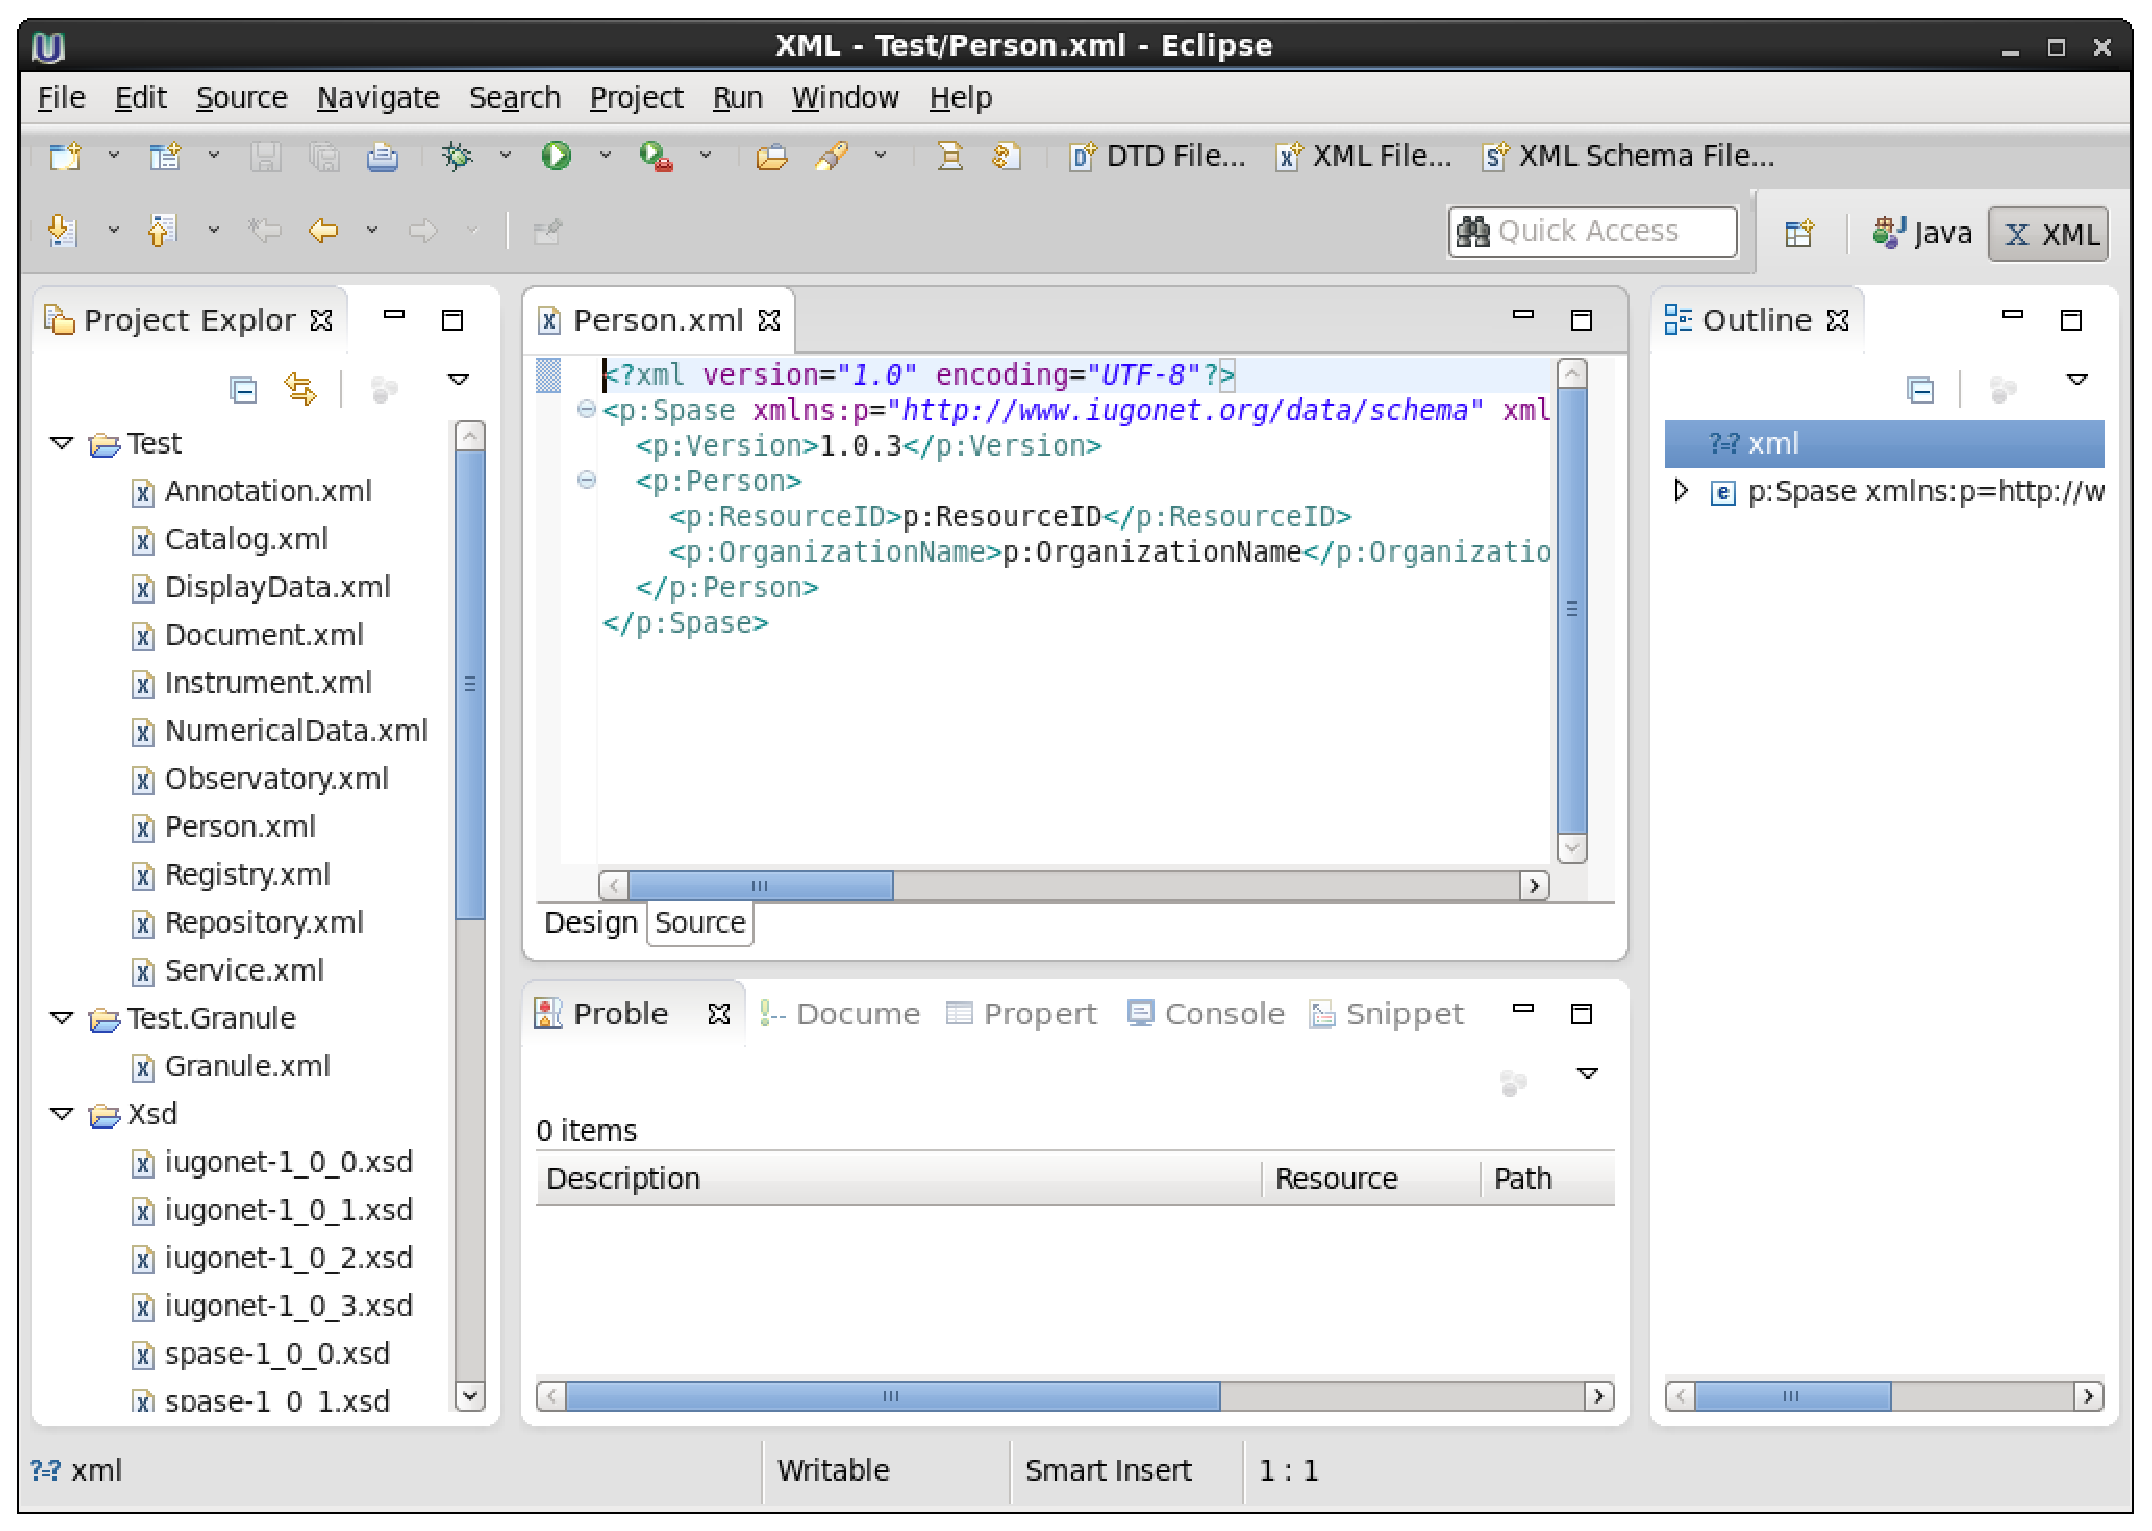
\includegraphics[width=12cm]{images/IugonetMetadataEditor3.eps}
}
\caption{Person.xml編集画面(Sourceタブ選択時)。図\ref{IugonetMetadataEditor2}のDesignタブ上で必要項目を埋めていけば、
この様に自動的にXML形式で記述されます。Sourceタブ上ではXMLの確認のみ行い、直接編集することは控えます。}
\label{IugonetMetadataEditor3}
\end{center}
\end{figure}

\begin{enumerate}
\item 最初は Spase の子要素として Catalog が選択されているので、Catalog 欄で右ク
リックすると、\colorbox[gray]{0.8}{Replace With}というツールバーが出るので、その中から編集したい子要素
(例えば \colorbox[gray]{0.8}{Observatory})を選択します(Space 欄で右クリック して、 \colorbox[gray]{0.8}{Add Child} の中から
必要な子要素を選択して追加した後、Catalog 欄で右クリックして\colorbox[gray]{0.8}{Remove} を選択、消去
しても同じ)。ここで、選択可能な子要素は、SPASE モデルで推奨・必須とされているメタ
データのカテゴリーです。それは、Catalog, DisplayData, Granule, Instrument,
NumericalData, Observatory, Person, Repository, Service などになります。
\item オプションの要素を足す場合は、親要素を右クリックして\colorbox[gray]{0.8}{Add Child} の中から選択、
もしくは今ある項目を右クリックして \colorbox[gray]{0.8}{Add Before} か \colorbox[gray]{0.8}{Add After}
 の中から選択します。
やり方は、①に準拠するので、上図を参照してください。
\item ある要素を消す場合は、その要素の欄で右クリックして \colorbox[gray]{0.8}{Remove} を選択します。
\item オプションの要素を足す場合は、今ある項目を右クリックして \colorbox[gray]{0.8}{Add Before} か
\colorbox[gray]{0.8}{Add After} の中から選択します。もしくは、親要素を右クリックして \colorbox[gray]{0.8}{Add Child}
 の中から選択します。やり方は、①に準拠するので、上図を参照してください。
\item NumericalData/Parameter の必須子要素として Field がデフォルトで選ばれてい
ますが、これは右クリックして\colorbox[gray]{0.8}{Replace With} の中から適当なもの(例えば \colorbox[gray]{0.8}{
Particle})に変
更できます。やり方は、①に準拠するので、上図を参照してください。
\item xsi:schemaLocation の値がローカルなスキーマファイルを指している場合(例え
ば、../../iugonet-1\_0\_0.xsd 等) 、Git リポジトリへ提出する前に
http://www.iugonet.org/data/schema/iugonet.xsd へ変更してください。
\item IUGONET 開発者が利用して気になったところ[いわゆる経験談]
(今後のメタデータファイルの作成時の参考にしてください。)
\begin{itemize}
\item オプションの要素を入れる位置が決まっているらしい。例えば、ResourceHeader でAcknowledgement を入れようとすると、Description のところで \colorbox[gray]{0.8}{Add After}
 とするか、Contact のところで \colorbox[gray]{0.8}{Add Before} としないと選択肢として出てこない。(親要素の欄で右クリックして \colorbox[gray]{0.8}{Add Child} から選択すればよいです)
\item ResourceHeader/Contact/Role ところで、指定された値の候補から選ぶ以外にも書き込めてしまうが... 。(SPASE、あるいはIUGONETで推奨されている項目以外は書かないようにしてください。不明な点はIUGONET の担当者まで)
\item 要素数が増えて画面に表示しきれなくなった場合、スクロールバーで最下部のほうを見ると、要素名は表示されるものの要素の値は表示されない。左クリックで入っている値がわかる。(※ Mac 版のみの現象らしいです。現在のところ対処方法は不明です)
\end{itemize}
\end{enumerate}

\begin{figure}[H]
\begin{center}
\fbox{
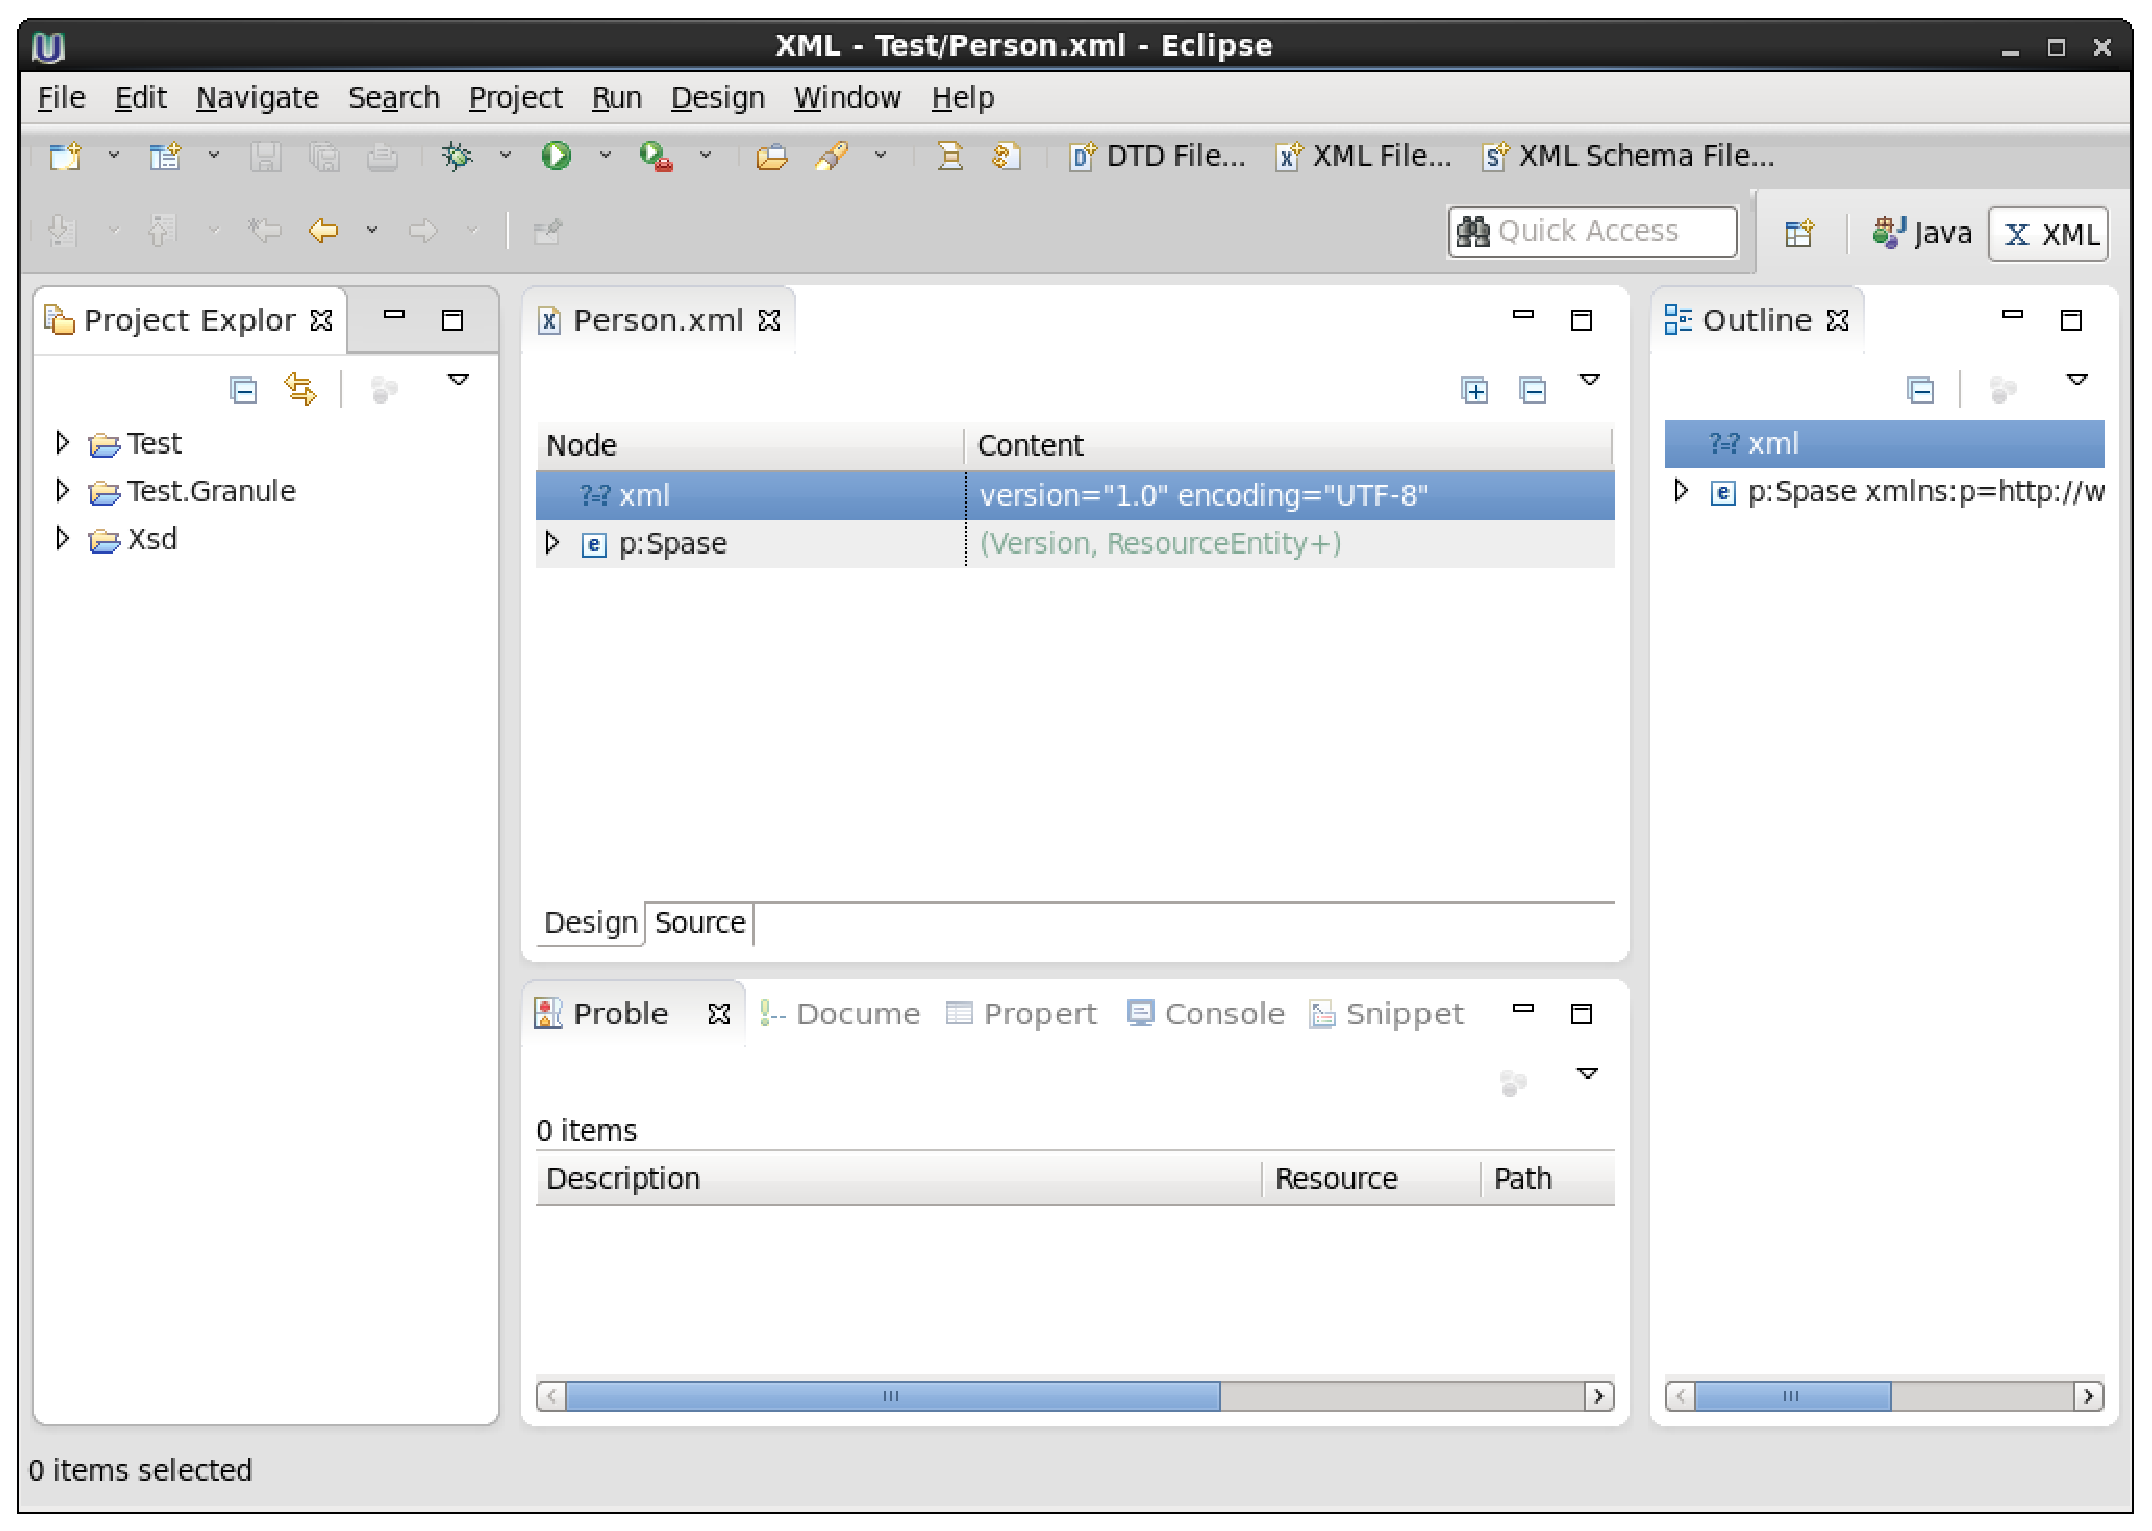
\includegraphics[width=12cm]{images/IugonetMetadataEditor1.eps}
}
\caption{6}
\label{6}
\end{center}
\end{figure}

\begin{figure}[H]
\begin{center}
\fbox{
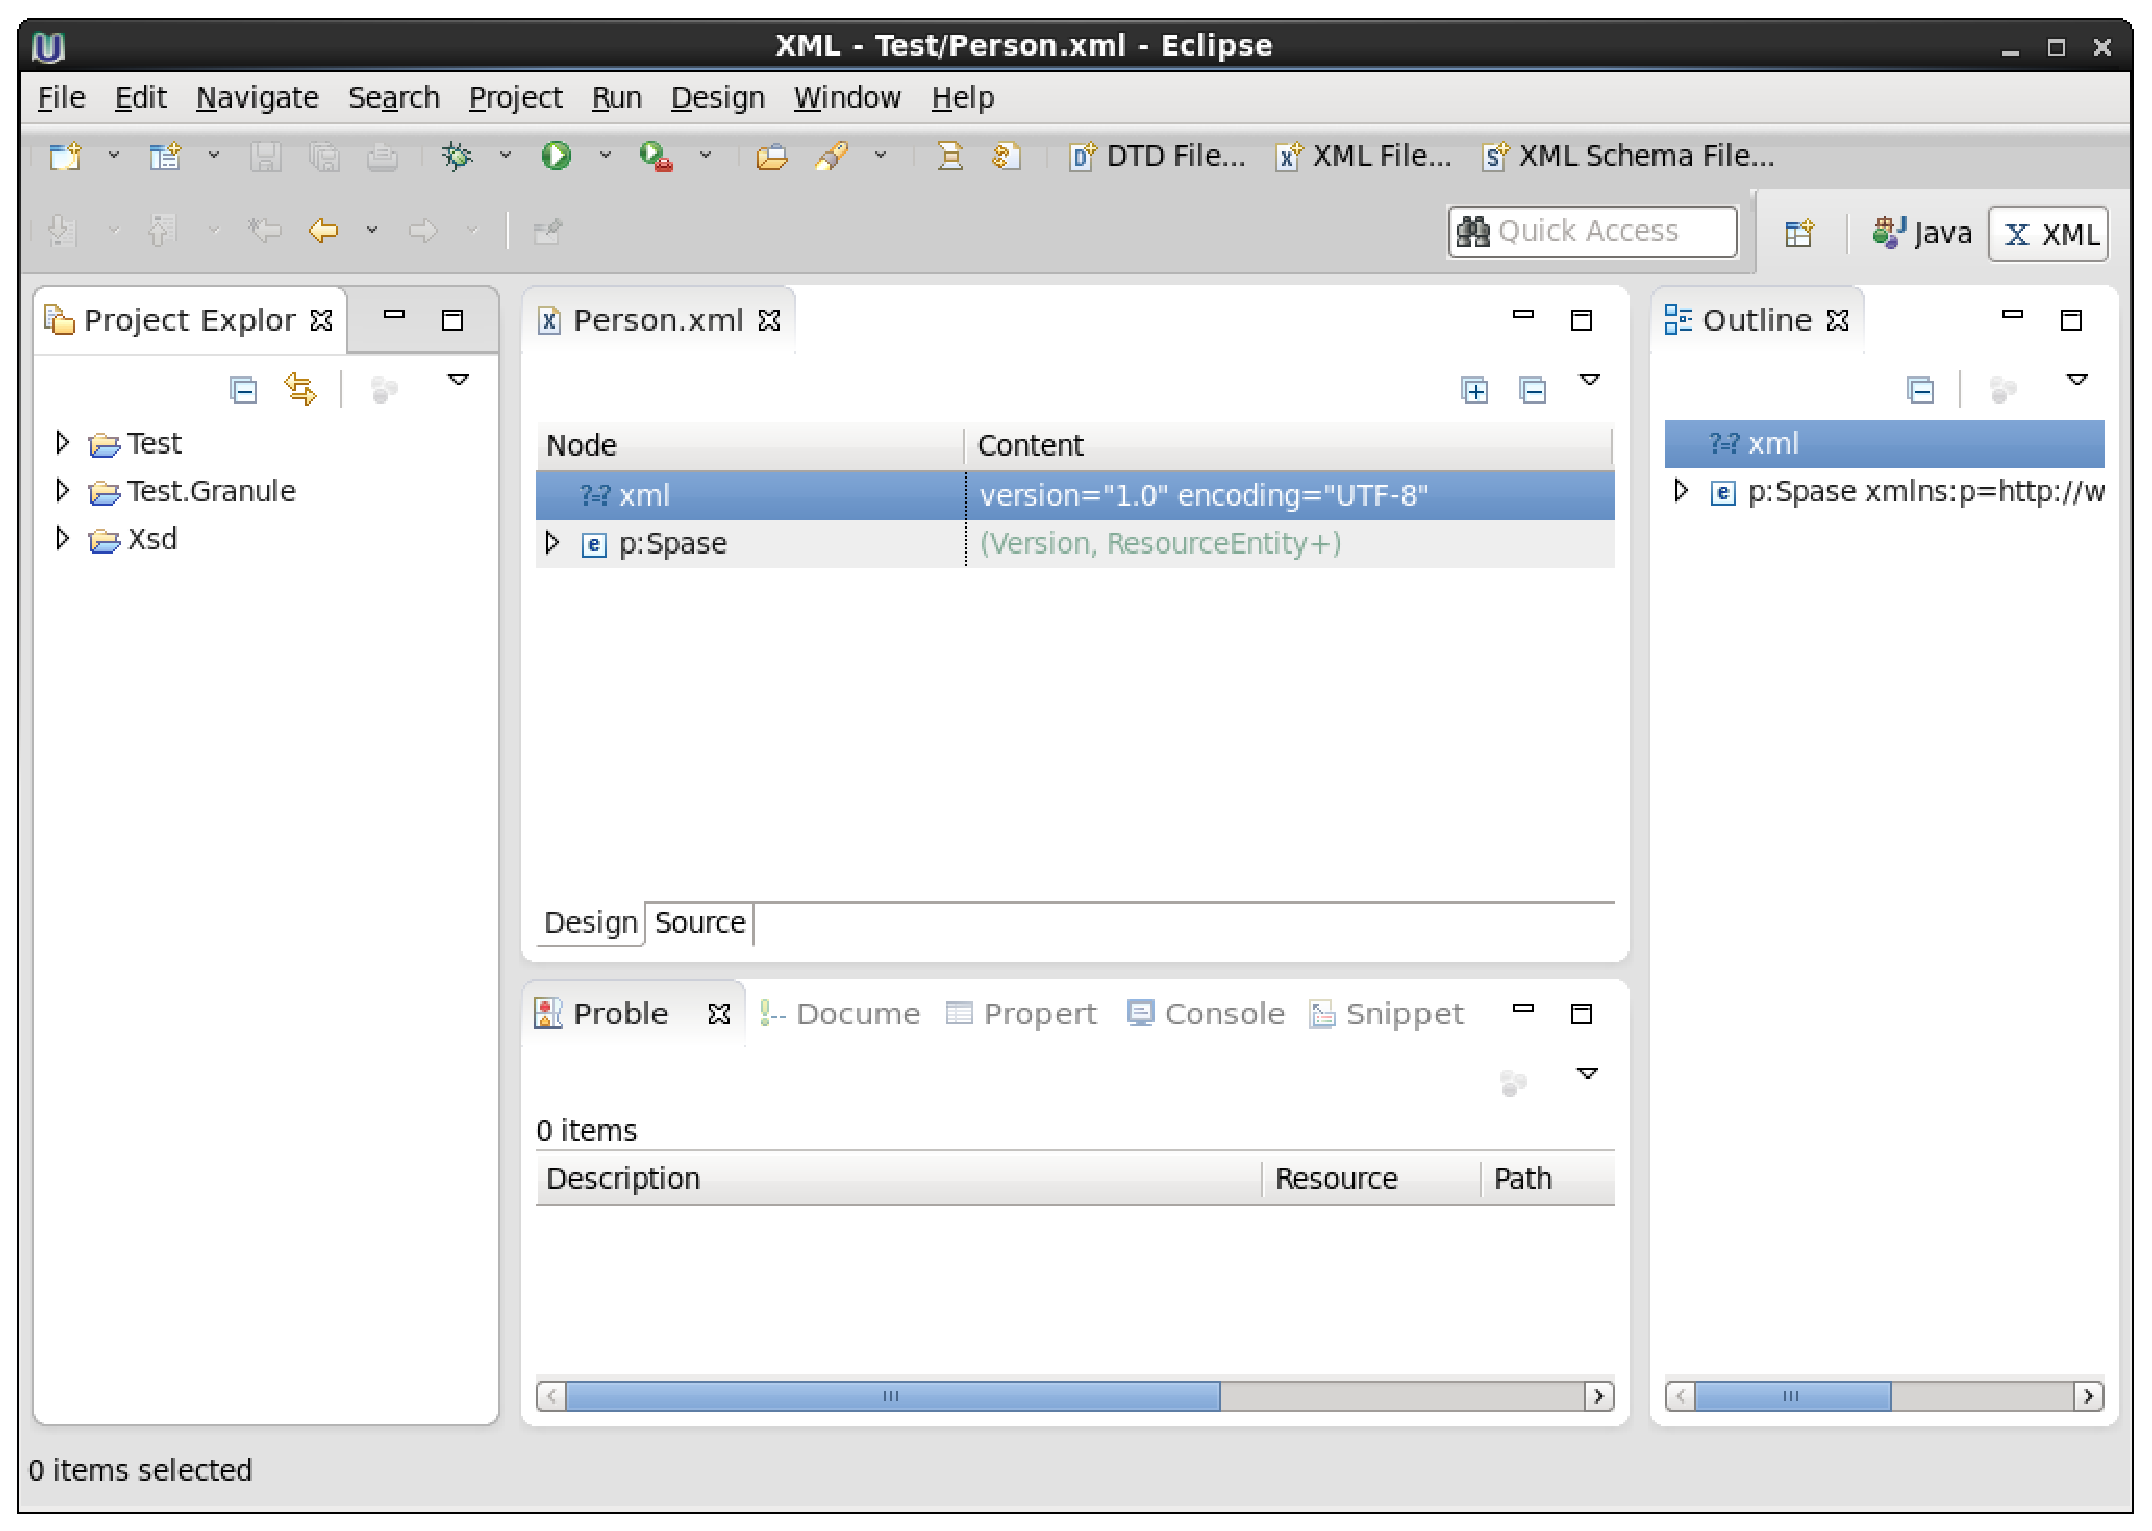
\includegraphics[width=12cm]{images/IugonetMetadataEditor1.eps}
}
\caption{7}
\label{7}
\end{center}
\end{figure}

\subsection{フォルダ(ディレクトリ)の追加}
\begin{enumerate}
\item ツールバーで \colorbox[gray]{0.8}{File} (エクスプローラーで右クリックでもよい) $\rightarrow$ 
\colorbox[gray]{0.8}{New} $\rightarrow$ \colorbox[gray]{0.8}{Folder}
の順に選択すると、ダイアログ(New Folder)が立ち上がります。
\item Folder
\begin{itemize}
\item Enter or select the parent folder: 親になるフォルダを選択します(もしくは直接入力する)。
\item Folder name: 新しく作るフォルダ名を入力します。
\item Finish をクリックすると、エクスプローラーに新しいfolder が現れます。
\end{itemize}
\end{enumerate}

\subsection{メタデータの簡易チェック}
Project Explore でメタデータを右クリックし \colorbox[gray]{0.8}{Validate} を選択することで、メタデータがIUGONETスキーマに適合しているかどうかをチェックすることができます。また、ディレクトリを右クリックして \colorbox[gray]{0.8}{Validate} を選択した場合、ディレクトリ内の全メタデータがチェックされます。エラーがある場合はProblemsタブにエラーが表示される他、Project Explore 上にバツ印がつきます。

\begin{figure}[H]
\begin{center}
\fbox{
\includegraphics[width=12cm]{images/IugonetMetadataEditor4.eps}
}
\caption{メタデータの簡易チェック (Problemsタブにエラーメッセージが表示) }
\label{IugonetMetadataEditor4}
\end{center}
\end{figure}

ただしスキーマのバージョンまで厳しくチェックしてしまうため、メタデータの version の値がwebページにおける最新版(ver1.0.4, 2014年11月現在) 以外を指定している場合、エラーになってしまいます。これは xsi:schemaLocation で指定した http://www.iugonet.org/data/schema/iugonet.xsd を参照しているためです。IUGONETでは{\bf ver1.0.3以降を推奨}としているため、ver1.0.3でエラーが出る場合でも問題はなく、無視して構いません。




